\documentclass[10pt,aspectratio=169]{beamer}
\usetheme{Madrid}
\usecolortheme{seahorse}

% Packages
\usepackage{graphicx}
\usepackage{booktabs}
\usepackage{tikz}
\usetikzlibrary{shapes.geometric, arrows.meta, positioning}
\usepackage{amsmath}
\usepackage{amssymb}
\usepackage{ragged2e}

% Force Beamer lists and text to be fully justified
\renewcommand{\raggedright}{\justifying}

% Custom Colors (Modern Royal Blue and Charcoal)
\definecolor{primaryblue}{RGB}{26, 54, 93}
\definecolor{accentblue}{RGB}{49, 130, 206}
\definecolor{charcoal}{RGB}{45, 55, 72}
\setbeamercolor{palette primary}{bg=primaryblue, fg=white}
\setbeamercolor{palette secondary}{bg=accentblue, fg=white}
\setbeamercolor{palette tertiary}{bg=charcoal, fg=white}
\setbeamercolor{titlelike}{parent=palette primary}

% Document Metadata
\title[Optimizing Incident Management]{Optimizing Incident Management Systems}
\subtitle{An Operations Research \& Machine Learning Approach}
\author[Divagar, Abhishek, Prem]{
    \textbf{Divagar S} \quad (CB.SC.U4AIE23223) \\
    \textbf{Abhishek Pandey} \quad (CB.SC.U4AIE23205) \\
    \textbf{Prem} \quad (CB.SC.U4AIE23241)
}
\date{\today}

\begin{document}

% 1. Title Slide
\begin{frame}
    \titlepage
\end{frame}

% 2. Problem Statement
\begin{frame}{Problem Statement}
    \begin{itemize}
        \item \textbf{Inefficient Ticket Routing:} Incident routing in support systems is often handled manually or via static rules, leading to processing bottlenecks.
        \item \textbf{Resolver Burnout:} Uneven workload distribution among the 9 active resolvers causes high queue times and resolver fatigue.
        \item \textbf{SLA Violations:} High-priority incidents suffer from delayed assignments, violating Service Level Agreements (SLAs).
        \item \textbf{Low Customer Satisfaction:} The average customer satisfaction is currently \textbf{3.23 / 5}, highlighting the need for process optimization.
    \end{itemize}
\end{frame}

% 3. Objectives
\begin{frame}{Objectives}
    \begin{block}{Primary Goal}
        Optimize the end-to-end incident management workflow to improve system throughput and customer experience.
    \end{block}
    \begin{columns}[T]
        \begin{column}{0.5\textwidth}
            \textbf{Operational Efficiency}
            \begin{itemize}
                \item Minimize total incident resolution time.
                \item Minimize SLA violation rate.
            \end{itemize}
        \end{column}
        \begin{column}{0.5\textwidth}
            \textbf{Resource \& Quality Management}
            \begin{itemize}
                \item Balance workloads across resolvers.
                \item Maximize customer satisfaction scores.
            \end{itemize}
        \end{column}
    \end{columns}
\end{frame}

% 4. Dataset Overview
\begin{frame}{Dataset Overview}
    \begin{columns}[T]
        \begin{column}{0.55\textwidth}
            \textbf{Process Mining Event Log - Incident Management} \\
            Work with a realistic event log for incident management.
            \vspace{0.2cm}
            
            \textbf{About the Dataset:} \\
            {\footnotesize This realistic incident management event log simulates a common IT service process and includes key inefficiencies found in real-world operations. You'll uncover SLA violations, multiple reassignments, bottlenecks, and conformance issues---making it an ideal dataset for hands-on process mining, root cause analysis, and performance optimization exercises.}
        \end{column}
        \begin{column}{0.45\textwidth}
            \centering
            \small
            \begin{table}[]
                \centering
                \begin{tabular}{ll}
                    \toprule
                    \textbf{Metric} & \textbf{Value} \\
                    \midrule
                    Total Events & 242,901 \\
                    Unique Cases & 31,588 \\
                    Resolvers & 9 \\
                    Priorities & High, Med, Low \\
                    Avg. CSAT & 3.23 / 5.00 \\
                    \bottomrule
                \end{tabular}
            \end{table}
        \end{column}
    \end{columns}
\end{frame}

% 5. Data Preprocessing Flowchart
\begin{frame}{Data Preprocessing Flow}
    \centering
    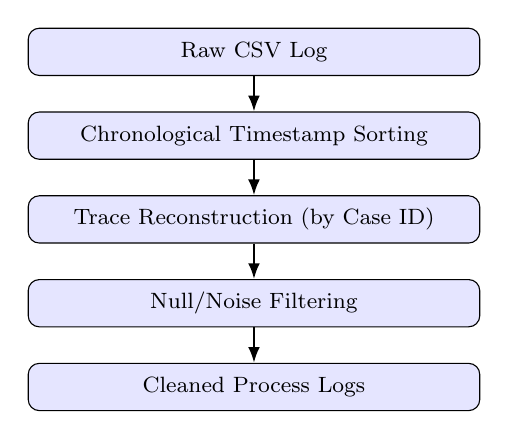
\begin{tikzpicture}[
        node distance=0.45cm,
        every node/.style={fill=white, font=\footnotesize},
        align=center
    ]
        % Style definitions
        \tikzstyle{block} = [rectangle, draw, fill=blue!10, text width=5.5cm, text centered, rounded corners, minimum height=0.6cm]
        \tikzstyle{line} = [draw, -{Latex[length=2mm]}, thick]

        % Nodes (Vertical Flow to fit slide height perfectly)
        \node [block] (raw) {Raw CSV Log};
        \node [block, below=of raw] (sort) {Chronological Timestamp Sorting};
        \node [block, below=of sort] (trace) {Trace Reconstruction (by Case ID)};
        \node [block, below=of trace] (clean) {Null/Noise Filtering};
        \node [block, below=of clean] (final) {Cleaned Process Logs};

        % Lines
        \path [line] (raw) -- (sort);
        \path [line] (sort) -- (trace);
        \path [line] (trace) -- (clean);
        \path [line] (clean) -- (final);
    \end{tikzpicture}
\end{frame}

% 6. Feature Extraction
\begin{frame}{Feature Extraction}
    To feed both machine learning and optimization models, we extract three categories of features:
    \begin{itemize}
        \item \textbf{Temporal Features (Durations):}
            \begin{itemize}
                \item \textbf{Queue Time ($W_{q}$):} Time from ticket assignment to WIP (work-in-progress).
                \item \textbf{Service Time ($S$):} Time from WIP to ticket solution/escalation.
                \item \textbf{Total Cycle Time ($T$):} Full duration from creation to closure.
            \end{itemize}
        \item \textbf{Categorical Context:}
            \begin{itemize}
                \item Ticket Priority, Issue Type, and Report Channel.
            \end{itemize}
        \item \textbf{Resource Performance Metrics:}
            \begin{itemize}
                \item Resolver throughput rate ($\mu_{i,j}$) and workload backlog size ($W_i$).
            \end{itemize}
    \end{itemize}
\end{frame}

% 7. Methodology
\begin{frame}{Methodology}
    \centering
    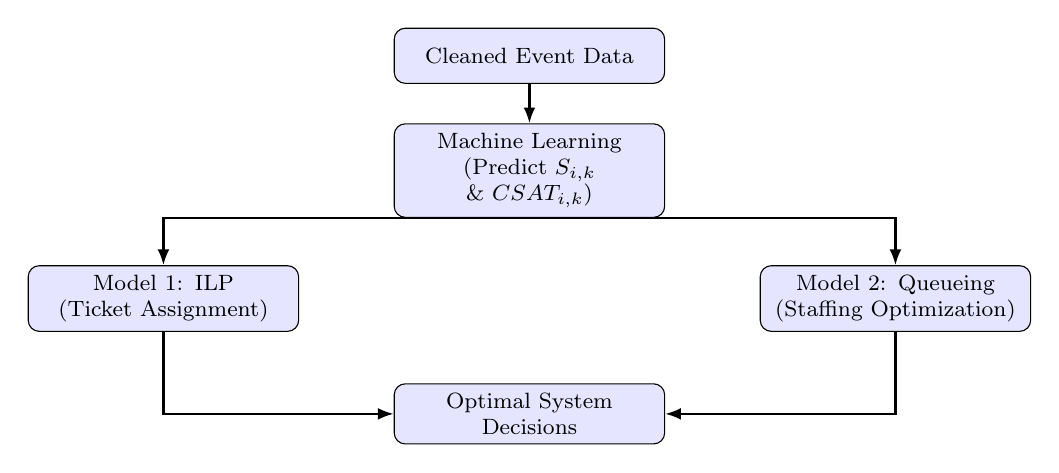
\begin{tikzpicture}[
        node distance=0.5cm and 0.8cm,
        every node/.style={font=\footnotesize},
        align=center
    ]
        \tikzstyle{block} = [rectangle, draw, fill=blue!10, text width=3.2cm, text centered, rounded corners, minimum height=0.7cm]
        \tikzstyle{line} = [draw, -{Latex[length=2mm]}, thick]

        % Hierarchical Vertical Layout to prevent overflow
        \node [block] (input) {Cleaned Event Data};
        \node [block, below=of input] (ml) {Machine Learning\\(Predict $S_{i,k}$ \& $CSAT_{i,k}$)};
        
        \node [block, below left=of ml, xshift=-0.4cm, yshift=-0.1cm] (opt1) {Model 1: ILP\\(Ticket Assignment)};
        \node [block, below right=of ml, xshift=0.4cm, yshift=-0.1cm] (opt2) {Model 2: Queueing\\(Staffing Optimization)};
        
        \node [block, below=of ml, yshift=-1.6cm] (output) {Optimal System\\Decisions};

        \path [line] (input) -- (ml);
        \path [line] (ml.south) -| (opt1.north);
        \path [line] (ml.south) -| (opt2.north);
        \path [line] (opt1.south) |- (output.west);
        \path [line] (opt2.south) |- (output.east);
    \end{tikzpicture}
\end{frame}

% 8. Model 1: Integer Linear Programming (ILP)
\begin{frame}{Model 1: Prescriptive Ticket Assignment (ILP)}
    \textbf{Optimal Ticket-to-Resolver Matching}
    \begin{itemize}
        \item \textbf{Purpose:} Assign incoming incidents to the 9 resolvers in real-time, minimizing resolution time and keeping workloads balanced.
        \item \textbf{Optimization Steps:}
            \begin{enumerate}
                \item Predict service time ($S_{i,k}$) for candidate resolver $i$ and ticket $k$ using regression.
                \item Query current backlog workload ($W_i$) for all active resolvers.
                \item Construct the ILP coefficient matrix based on predicted service times and priorities.
                \item Run the ILP solver at each assignment decision epoch to compute optimal assignments.
            \end{enumerate}
    \end{itemize}
\end{frame}

% 9. Model 2: Jackson Queueing Network
\begin{frame}{Model 2: Tiered Staffing Optimization}
    \textbf{Queuing Network Analysis}
    \begin{itemize}
        \item \textbf{Purpose:} Model Level 1, 2, and 3 tiers as a network of queues to optimize the number of agents needed to meet target response times.
        \item \textbf{Optimization Steps:}
            \begin{enumerate}
                \item Estimate Poisson arrival rates ($\lambda$) and exponential service rates ($\mu$) for each tier.
                \item Formulate the system as a Jackson Network with routing probabilities ($P_{1 \to 2}$ escalation rates).
                \item Solve the multi-server queue equations ($M/M/c$) for steady-state performance.
                \item Optimize the count of active resolvers ($c_1, c_2, c_3$) to minimize operating costs while keeping average wait time below SLA limits.
            \end{enumerate}
    \end{itemize}
\end{frame}

% 10. Objective Function
\begin{frame}{Objective Function}
    We formulate a multi-objective function to balance speed, customer satisfaction, and resolver workloads:
    
    \begin{block}{Weighted Objective Function}
        \[
        \min \quad Z = \alpha \sum_{k \in K} \sum_{i \in I} P_k \cdot S_{i,k} \cdot x_{i,k} - \beta \sum_{k \in K} \sum_{i \in I} CSAT_{i,k} \cdot x_{i,k} + \gamma \cdot \sigma^2_{\text{workload}}
        \]
    \end{block}
    \vspace{0.2cm}
    \textbf{Where:}
    \begin{itemize}
        \item $\sum P_k \cdot S_{i,k} \cdot x_{i,k}$: Total priority-weighted resolution time (to minimize).
        \item $\sum CSAT_{i,k} \cdot x_{i,k}$: Total expected customer satisfaction (to maximize).
        \item $\sigma^2_{\text{workload}}$: Variance of workloads among resolvers (to minimize for balance).
        \item $\alpha, \beta, \gamma$: Scaling weights adjusting priorities.
    \end{itemize}
\end{frame}

% 11. Constraints and Decision Variables
\begin{frame}{Constraints and Decision Variables}
    \textbf{Decision Variable:}
    \[
    x_{i,k} = \begin{cases} 1 & \text{if ticket } k \text{ is assigned to resolver } i \\ 0 & \text{otherwise} \end{cases}
    \]

    \textbf{Constraints:}
    \begin{itemize}
        \item \textbf{Single Assignment Constraint:} Each incident must be assigned to exactly one resolver.
            \[ \sum_{i \in I} x_{i,k} = 1 \quad \forall k \in K \]
        \item \textbf{Resolver Capacity Constraint:} No resolver can exceed their maximum workload capacity $C_i$.
            \[ W_i + \sum_{k \in K} x_{i,k} \le C_i \quad \forall i \in I \]
        \item \textbf{Tier Routing Constraint:} Tickets must be assigned only to resolvers active in the correct tier (L1, L2, L3).
    \end{itemize}
\end{frame}

% 12. Evaluation Metrics
\begin{frame}{Evaluation Metrics}
    \begin{columns}[T]
        \begin{column}{0.5\textwidth}
            \textbf{Operations Research Metrics}
            \begin{itemize}
                \item \textbf{Average Cycle Time:} Mean resolution time of tickets.
                \item \textbf{SLA Compliance Rate:} Percentage of incidents resolved within deadline.
                \item \textbf{Workload Gini Coefficient:} Metric for measuring workload distribution equality.
            \end{itemize}
        \end{column}
        \begin{column}{0.5\textwidth}
            \textbf{Machine Learning Metrics}
            \begin{itemize}
                \item \textbf{Mean Absolute Error (MAE):} On predicted service times.
                \item \textbf{R-squared ($R^2$):} Variance explained in satisfaction score predictions.
            \end{itemize}
        \end{column}
    \end{columns}
\end{frame}

% 13. Tools and Technology
\begin{frame}{Tools and Technology}
    \begin{itemize}
        \item \textbf{Programming Language:} Python 3.x
        \item \textbf{Data Manipulation:} Pandas, NumPy (for data processing)
        \item \textbf{Predictive Modeling:} Scikit-Learn, LightGBM (for service time and CSAT predictions)
        \item \textbf{Mathematical Optimization Solvers:} PuLP / Gurobi / SciPy (for ILP optimization)
        \item \textbf{Simulation Engine:} SimPy (for queueing network discrete event simulation)
        \item \textbf{Typesetting \& Graphics:} \LaTeX / Beamer (slides), TikZ (flowcharts)
    \end{itemize}
\end{frame}

% 14. End Slide
\begin{frame}
    \centering
    \Huge \textbf{\color{primaryblue}{Thank You}} \\
    \vspace{0.5cm}
    \large Questions \& Comments
\end{frame}

\end{document}
